\documentclass[html]{report}    % Specifies the document style.
\usepackage{graphicx}
\usepackage{verbatim}
\usepackage{amsmath}  % allows to use some of math functions
                           % The preamble begins here. 
\title{Multi-Agent Systems Project}  % Declares the document's title. 
\author{Panagiotis Chatzichristodoulou, Kirill Tumanov} 
%\date{November 29,2013}   % Deleting this command produces today's date.

\begin{document}           % End of preamble and beginning of text.

\maketitle                 % Produces the title.
\section{Introduction}
\subsection{Abstract}
This paper addresses the implementation of an intelligent negotiation agent. Furthermore, it discusses and analyses the results obtained from the experiments that were performed. 
\subsection{Project Analysis}
The agents created are based on the negotiation platform genius. ~\cite{genius} . The genius platform released it's first demo edition from Delft University on May 14th 2009. It introduces an environment where agents can negotiate over different domains,  discrete or continuous. Genius is the standard in the agent negotiation domain platform. The work was performed as a practical part of the Multiagent Systems course at Maastricht University. 

\subsection{Agent models}
Each agent can consist of 4 different models:
\begin{itemize}
  \item The bidding strategy
  \item The acceptance strategy
  \item The Opponent strategy
  \item The Opponent model   
\end{itemize}
The agents in the genius platform can either be standalone agents , or agents that belong to the BOA framework. A standalone agent is usually a single java file having all the models there. Some helper classes can exist outside of the main agent class. A BOA agent implements the four needed models independently , and that makes a BOA agent more versatile and easier to implement, due to the modularity of its architecture. In our implementation we chose a BOA agent and used the genius platform to create our final agent that consists of those four parts. The figure below depicts how the four different models cooperate to output a bid or an acceptance decision.
\begin{figure}[htbp]
	  \caption{Cooperation between four models,\newline \it{BOA framework}}
	  \centering
	    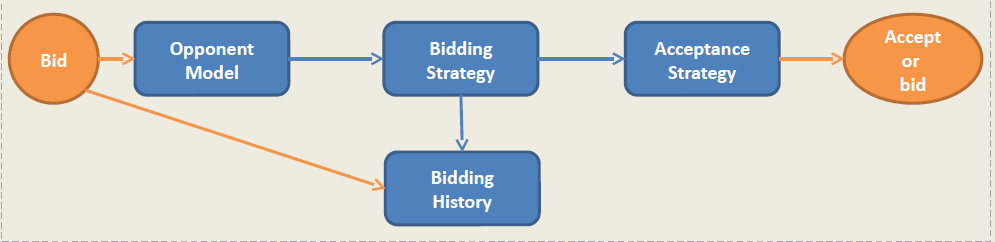
\includegraphics[width=1\textwidth]{fourmodels}
	  \label{1}
\end{figure}
%\pagebreak


\subsection{Agent type}
The agent that is implemented in this paper, is self interested . That is an agent that seeks to optimize its utility without taking into account the opponent's utility, or the social welfare. Furthermore, it takes into account the discount factor, and will not negotiate for too long. That way, it will receive as high utility as possible most of the time.

\section{Bids Offering Strategy}
Agent's bid offering strategy was implemented as time-dependent (TD). The NegoAgent\_TDOffering.class requires two user parameters: $P_{min}$ and $P_{max}$ which specify the lower and upper bounds for the bids agent is to propose. In the current version of the agent these values were kept equal to $0$ and $0.99$ respectfully. No experimentation was done on changing these values, it may be the case that some alterations in specific negotiation domains are beneficial, however this topic is left for an additional research.

Offering strategy introduces two methods used in the agent: \texttt{isNash()} and \texttt{countUniqueBids()}. First one is a simple implementation of the two-factor (due to the number of negotiating parties) maximization algorithm. An idea behind it is in finding a Nash equilibrium point, there none of the parties can obtain a higher utility at no cost to any other party. This particular implementation does not claim to be optimal, but it produced sufficiently good results for the agent at this stage of development. The pseudo-code of the  \texttt{isNash()} method is given as follows:
\begin{verbatim}
double nashsum;
boolean isNash(){
    bid = getOpponentLastBid();		
    if (bid != null) {
        temp = bid.getMyUtility() + bid.getOppenentUtility();
        if (temp < nashsum && bid.getOppenentUtility() < bid.getMyUtility())
            return true;			
        nashsum = temp;
    }		
    return false;
}
\end{verbatim}
Here \texttt{nashsum} stores a previously found maximum combined utility result to compare the last opponent bid against. When \texttt{nashsum} becomes less than the last bid combined utility, then Nash is found and true is returned. An additional limit in the opponent's and agent's utilities is set to ensure, that Nash bid was proposed by the opponent, and not by the agent itself.

The second method \texttt{countUniqueBids()} is implemented to find and count all the opponent's non-equal bids as well as calculate a total sum of all proposed bids. A pseudo-code of the method is given below.
\begin{verbatim}
uniquebids;
double bidsum;
countUniqueBids() {
    int count = 0;
    bid = getOpponentLastBid();	
    if (getOpponentBidHistory().size() == 1) {
        uniquebids.add(bid.getMyUtility());
        bidsum += bid.getMyUtility();
    }
    else {
        for (uniquebid : uniquebids) {
            if (uniquebid != bid.getMyUtility()) {
                count ++;
            }
        }
        if (count == uniquebids.size()) {
            uniquebids.add(bid.getMyUtility());
            bidsum += bid.getMyUtility();
        }
    }
}  
\end{verbatim}
This method is supposed to be called every time an opponent proposes a new bid. As a result a list of \texttt{uniquebids} representing agent's utility values, \texttt{bidsum} value of all bids and \texttt{count} are stored and used for further calculations.

The main procedure of the agent's bidding strategy is \texttt{determineNextBid()} which relies on a time-dependent function \texttt{p(t)}. For this work we introduce a novel TD function, results of which are determined by the values received from the methods described above. The following is a pseudo-code of the \texttt{p(t)} implementation.
\begin{verbatim}
int bidsThreshold ;
double timeThreshold;
double p(double t) {
    countUniqueBids();
    double ft = calculateF(t);
    double time = getTime();
    if (getNumberOfPossibleBids() < bidsThreshold) {
        if (time > timeThreshold) {
            ft += getOpponentLastBid.getMyUtil()/(1 - time);
        }
    }
    pt = Pmin + (Pmax - Pmin) * (1 - ft);
    return pt;
}
\end{verbatim}
Here \texttt{pt} is used only for adjustment of the ft result based on the $P_{min}$ and $P_{max}$ bid bounds discussed at the beginning of the section. The most interesting part is a calculation of \texttt{ft}:
\begin{equation} \label{1}
	f(t) = \begin{cases}
			df(\sin(-n\cdot e^{t\cdot df})+(\frac{1}{df}-1))\cdot\log(t\cdot df+1)\cdot\frac{sum}{ubs}t &\text{if ubs$>$1 and !isNash(),}\\
			\frac{df}{2}(\sin(-n\cdot e^{t\cdot\frac{df}{2}})+(\frac{2}{df}-1))\cdot\log(t\cdot \frac{df}{2}+1)\cdot\frac{sum}{ubs}t &\text{if ubs$>$1,}\\
			df(\sin(-n\cdot e^{t\cdot df})+(\frac{1}{df}-1))\cdot\log(t\cdot df+1) &\text{otherwise.}
			\end{cases}
\end{equation}
where $df$ - a division factor in a range $\{0\dots1\}$, $n$ - number of issues negotiation about, $t$ - representation of time in a range $\{0\dots1\}$, $sum$ - a total sum of all opponent's bids at the moment of $t$ (afore-referred as a \texttt{bidsum}), $ubs$ - number of unique opponent's bids at the moment of $t$ (a size of an afore-referred list of \texttt{uniquebids}).

The function $f(t)$ was designed so that it allows modification of bid offering dependent on the negotiation status. If opponent proposes more non-equal bids of a decent utility for an agent, then agents offers new bids more cautious - simulation of waiting for the best opponent's offer. On contrary, when opponent proposes a few non-equal bids, agent tries to provoke an opponent for cooperation, by offering more new bids. In addition, a fact of Nash equilibrium reach by an opponent is treated as a trigger to loose agent's own offering, and to start biding more actively. It is done in order to prevent an opponent from unnecessary utility losses, whilst it is likely that agent's own score is not going to be lowered. Finally, increase of $t$ during the negotiation process unveils more new bids to offer, and $n$ ensures that the offering will be domain-dependent.

Referring back to the pseudo-code of \texttt{p(t)}, in case of a very limited utility space (\texttt{getNumberOfPossibleBids() $<$ bidsThreshold}) and negotiation time running out (\texttt{time > timeThreshold}), agent begins to concede by increasing the $f(t)$ value proportionally to the remaining time $(1-t)$. This allows to reach an agreement, instead of loosing all the utility. However, note that when opponent follows a non-cooperative strategy, this approach will not be of help.                

\section{Acceptance Strategy}  
\subsection{Summary}                        
An acceptance strategy of the agent was based on the ABiNeS agent's ~\cite{abines} acceptance strategy. This module introduces an acceptance threshold $\ell$. The value of $\ell$ corresponds to the agents concession degree and is modified during the negotiation. This change is based on the previous results of the negotiation as well as on the domain.

The agent is build as a self-interested agent and will be more concessive as the deadline of $t=1$ approaches. The acceptance threshold should always be higher than the utility agent can obtain at deadline. Therefore, the threshold should never be lower than the  \( Utility_{max} * discount_{time-1}  \) , where \( Utility_{max} \)  is the maximum utility the agent can receive without taking into account the discount factor. In contrast, if it takes the agent too long to reach an agreement, it may receive very low utility due to the influence of a discount factor even if the agreed outcome proposes a high utility. 

To address the issue factor $\lambda$ is introduced. It is used to balance between exploring and exploiting the negotiating partner. More formally, when time is smaller than $\lambda$, it should be modified to gradually converge to \( Utility_{max} * discount_{time-1}  \). So the $\ell$ is defined as follows:

\begin{equation} \label{2}
	\ell =	\begin{cases}
	    	u^m -(u^m-	u^md^t)(t/\lambda)^a  & \mbox{if } t \geq \lambda, \\
	   		u^m d^t & \mbox{if } t < \lambda.
			\end{cases}
\end{equation}

\begin{equation} \label{3}
	\lambda =	\begin{cases}
	   		  	\lambda = \lambda_0 + (1-\lambda_0)^b &  \mbox{if } t==0,\\
	       		 \lambda = \lambda + w(1-\lambda_0)\sigma^t & \mbox{if } 0<t\leq1.\\
				\end{cases}
\end{equation}
So as time increases, $\ell$ slowly decreases, and as time reaches $\lambda$, $\ell$ is set to \( Utility^{max}\cdot discount^{time}  \). Graphical representation of the process is presented on Fig.~\ref{1}. Here notable is that values of $b$ and $c$ define the curvature of nonlinear piece, specifically they set a lower bound of an acceptance threshold. This fact is crucial for the strategy's implementation, as both $b$ and $c$ values should be domain-dependent in order to adequately reflect the setup features and prevent early acceptance of non-desirable offers from an opponent. Generally~$b>1$~and~$c>1$.

\begin{figure}[htbp]
	\caption{Change of $\ell$ over time}
	\centering
	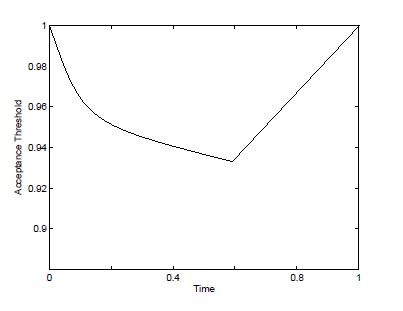
\includegraphics[width=0.5\textwidth]{ell}
	\label{2}
\end{figure}

\subsection{Acceptance Model}

Now that we have defined the environment, the acceptance condition is a function of the history of the previous negotiations, the current acceptance threshold, and the outcome of the negotiation at time $t$.

The agent will accept a proposal $\pi$ if he receives utility bigger than his current threshold, or his next-bid to propose utility.

\section{Opponent Model}  

An opponent model is based on the Hard-Headed Opponent Model of the genius-BOA framework.

Besides from the basic model, there are two extra components in the model.~\cite{anac2013}

\subsection{Simple Frequency}

The Simple frequency model only updates weights when the bid change often.
That means that the weights of the model are only changed when the opponents bids pass a certain numerical threshold.

\subsection{Distance of the opponent}

The opponent model also calculates a threshold that is used in the Acceptance Strategy and is based on the distance of the opponent.

{\bf The basic algorithm of the distance of the opponent is: }

DOUS = u$^m - firstOppBid \newline
calculate\ mean\ and\ variance\ foreach\ past\ bid\ where:\newline
firstOppBid< bidUtil<u^m \newline
use\ the\ (mean+dous)/2\ as\ a\ threshold\ value\ if\ time<.5 \newline
if(time<.5)\space return \ threshold \ else \ return \ 0$

The visualization of the DOUS distance would be:

\begin{figure}[htbp]
  \caption{The distance between the initial utilities of the agents}
  \centering
    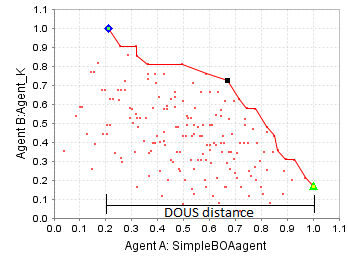
\includegraphics[width=0.5\textwidth]{dous}
    \label{3}
\end{figure}


The DOUS value is versatile, as it is not domain dependent.
As it is presented here, it can be implemented only on negotiations of two agents, but it can be expanded to multiple agent negotiations.
The threshold is outputted is weak threshold.
That is, if the value is smaller than the threshold, the bid is rejected. If the value is higher, we compare it with the normal threshold computed in the Acceptance Strategy.
This threshold ensures that the agents will reject points that are far from the Nash equilibrium.
After some time in the negotiation, the threshold is set to zero, because the agent needs to be more concessive as the negotiation approaches the deadline. 

\section{Binding the Modules}

It is useful to have a single-entity agent instead of several BOA components. In particular, \textit{Genius} allows single-entity agents run separate sessions against each other, and \textit{ANAC} competition uses this kind of agents in the tournament series. A single-entity agent may consist of numerous parts, however the one described in the paper is comprised of four main BOA components:
\begin{itemize}
	\item Bidding Strategy
	\item Acceptance Strategy
	\item Opponent Model
	\item Opponent Model Strategy
\end{itemize}

In order to bind all the modules together, a class that extended the BOA agent and passes each of the modules with it's parameters as parts of the agent should be created. Then it is necessary to override an \texttt{agentSetup()} method of the class. The pseudo-code of the overriden class is:

\begin{verbatim}
NegoAgent extends BOAagent {    
    @Override
    agentSetup(){
        OpponentModel om = new OpponentsModel(negotiationSession);
        OMStrategy oms = new BidStrategy(negotiationSession , om);
        OfferingStrategy offering = new NegoAgent_TDOffering(nego-
        tiationSession, om, oms, Pmax, Pmin);
        AcceptanceStrategy ac =  new AStrategy(negotiationSession,
        offering, a , b, c);
        setDecoupledComponents (ac, offering, om, oms );
    }
}
\end{verbatim}

\section{Results}

The agent implemented is a very-strong willed agent (Our agent beats them all!!). It will accept bids faster when the discount factor is big, and will negotiate for a long time when the discount is small. Its acceptance strategy with the weak threshold enable it to accept offers that are at least close to nash equilibrium, and as time approaches 1, it accepts more reasonable bids. Its bidding formula makes the agent extremely efficient at obtaining the best utility possible from strong willed opponents. The figures below show the results against a very good 2013 agent.


\section{Conclusion and further work}
Building a negotiating agent is a non-trivial matter, as the negotiation domains are practically infinite, as are the strategies that can be used. As the agent negotiation is a research field that has only been introduced recently, and as there are strategies that behave well given different domains there is a lot of research to be done , until we reach a universal strategy, or a strategy that works very well in all of the domains.


\begin{thebibliography}{}

\bibitem{abines} 
Hao J., Leung H.:
ABiNeS: An Adaptive Bilateral Negotiating Strategy over Multiple Items

\bibitem{anac2013} 
Something

\end{thebibliography}

\end{document}